As shown in section \ref{sec:alg}, multi-view deconvolution relies on 3D image stack convolutions with large kernels. In order to iterate towards an efficient design of multi-view deconvolution, this section will discuss model implementations and their benchmarks on hardware introduced in section \ref{sec:hw}. All of the model systems use synthetic data which is validated after each run upon consistency where appropriate. If not stated otherwise, the synthetic data has been generated in steps of powers of 2 in each dimension, so that each benchmark was run on $64x64x64$, $128x64x64$, $128x128x64$, \dots, $1024x1024x1024$ shaped datasets if possible.

\subsection{Single FFT}

As the heart of the application are FFT, there performance on CPU and GPU should be compared. For this, the most simple setup is used.

\begin{lstlisting}[caption={Single FFT on synthetic data performed on CPU in pseudo-code based on the \fftw{} syntax.},label={lst:single_fft_cpu}]
stack_f32 synthetic_data;

fftwf_plan plan = fftw_plan_dft_r2c(3,
                                    synthetic_data.shape(),
                                    synthetic_data.ptr(),
                                    synthetic_data.ptr(),
                                    FFTW_MEASURE);
//start timing
fftwf_execute(plan)
//end timing
\end{lstlisting}

Listing \ref{lst:single_fft_cpu} gives an overview on the syntax required to execute a \fftw{} 3D FFT on spatial domain data and whose result is written back to the same memory location in the frequency domain (in-place transform). The application programming interface (API) requires plan to perform the transform operation. According to the documentation \cite{fftw_manual}, the plan allocates additional memory for structures required during FFT execution. This global variable hence exerts a software design force on all clients to be aware of this behavior. Moreover, plans should be reused in order to prevent unnecessary reallocations. The equivalent implementation to perform the FFT on the \gpu{} is given in listing \ref{lst:single_fft_gpu}.\newline

\begin{lstlisting}[caption={Single FFT on synthetic data performed on GPU in pseudo-code based on the \cufft{} syntax.},label={lst:single_fft_gpu}]
stack_f32 synthetic_data;
float* device_ptr = 0;
cudaMalloc(device_ptr, sizeof(float)*synthetic_data.size());
cudaMemcpy(device_ptr, synthetic_data.ptr() , sizeof(float)*synthetic_data.size(), cudaHostToDevice);

cufftHandle plan;
cufftPlan3d(&plan,synthetic_data.shape(0),synthetic_data.shape(1),synthetic_data.shape(2),CUFFT_R2C);

//start timing
cufftExecR2C(plan, device_ptr, device_ptr);
//end timing

cudaMemcpy(synthetic_data.ptr(), device_ptr , sizeof(float)*synthetic_data.size(), cudaDeviceToHost);
\end{lstlisting}

Clearly, the offload model of having \gpu{} memory being separate from \cpu{} memory requires a lot more syntax than for plain \cpu{} use cases. However, the \cufft{} API is similar in nature to \fftw{} except the more stringent procedural approach (no functions with return values, rather than functions operating on structs). As \texttt{cudaMemcpy} is used to transfer data from host to device and back, this implementation is internally synchronized.\newline

\begin{figure}[h]
  \centering
  \hfill
  \begin{subfigure}[b]{0.45\textwidth}
    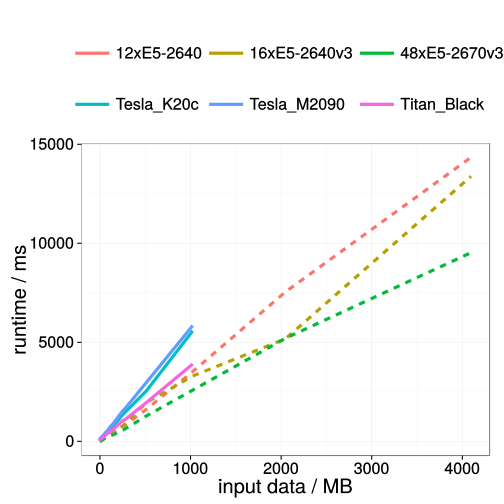
\includegraphics[width=\textwidth]{plots/synced_gpu_runtime}
    \caption{CUDA runtime}
    \label{fig:single_fft_runtime}
  \end{subfigure}%
  \hfill
  \begin{subfigure}[b]{0.45\textwidth}
    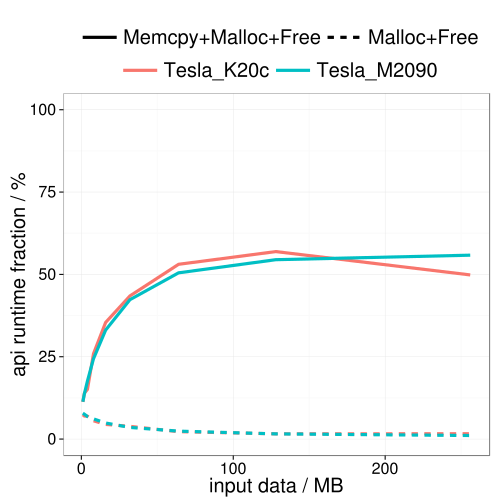
\includegraphics[width=\textwidth]{plots/synced_gpu_api_fractioninplace}
    \caption{CUDA API fraction}
    \label{fig:single_fft_api_fraction}
  \end{subfigure}
  \hfill
  \caption{Runtimes for single 3D FFT on synthetic data on \cpu{} with \fftw{} and on \gpu{} with \cufft{} (left, \ref{fig:single_fft_runtime}) and API time fraction of runtime dedicated to data (de-)allocation and/or data transfer (right, \ref{fig:single_fft_api_fraction}).}
  \label{fig:rt_single_fft}
\end{figure}

Figure \ref{fig:rt_single_fft} illustrates the runtime budget of an FFT transformation. Subfigure \ref{fig:single_fft_runtime} shows a linear rise in runtime with increasing input data. This is the behaviour expected from considerations of equation \ref{eq:fft_convol_complexity}. It is interesting to observed what fraction of this runtime is invested in data transfers. Figure \ref{fig:single_fft_api_fraction} hints to $\unit[50]{\%}$ of the total runtime is dedicated to data transfers. This implies, that if data transfer can be hidden or accelerated, this would beneficial for the entire algorithm.

\subsection{Batched FFTs}